% Errors

\chapter{Background}
\label{cha:background}

In this chapter, we present the tools and concepts employed throughout this project. We begin by introducing the Rocq Proof Assistant, highlighting the features that make it suitable for our implementation. We then describe the \gls{ssa} form, the intermediate representation family we use. Finally, we discuss the theoretical foundations of \gls{ra}, with particular attention to SSA programs.

\section{The Rocq Proof Assistant}

Rocq is an interactive proof assistant. It provides a specification language called Gallina, this language is used for defining functions, types, and proposition. It also provides a language for writing proofs, called Ltac, and finally a language for interacting with the Rocq kernel through commands, called Vernacular. It is also possible to extract Gallina definitions into optimized languages such as OCaml, Haskell or Lisp.

\subsection{Function Termination}
\label{subsec:funterm}

Recursive functions are typically defined using the \texttt{Fixpoint} keyword. With this keyword Rocq statically checks that, for each recursive call, there exists a structurally decreasing argument, guaranteeing termination by eventually reaching a base case.

Some recursive functions, however, do not conform to this criterion. Take for example the function for performing division by repeated subtraction:

\begin{lstlisting}[style=Rocq]
Fail Fixpoint div (a b : nat) : nat :=
  match b with
  | 0 => 0
  | _ =>
    if b <? a
    then 1 + div (a - b) b
    else 0
  end.
\end{lstlisting}

As we see, at line 6, we perform a recursive call, passing \texttt{(a - b)} as an argument. It is obvious that the argument decreases on each recursive call. However, Rocq cannot guess it, as it is only capable of identifying a decreasing argument if it is the parameter of a constructor. Because of that, the previous definition generates an error.
To solve such cases, in our project, we use two common workarounds.

% There are more, say that in this theses you only use these 2 workaround
The first approach we use is fuel-based recursion, it consists in adding an artificial decreasing argument, commonly named \texttt{fuel}, to the function signature.
Here is the division function with a definition that is accepted by Rocq:

\begin{lstlisting}[style=Rocq]
Fixpoint div (a b : nat) (fuel : nat) : nat :=
  match fuel with
  | 0 => 0
  | S fuel' =>
    match b with
    | 0 => 0
    | _ =>
      if b <? a
      then 1 + div (a - b) b
      else 0
    end
  end.
\end{lstlisting}

As we see, at line 4, we get the decremented value \texttt{fuel'}, this value is then passed as an argument in the recursive call at line 9.
Termination is guaranteed when \texttt{fuel} reaches zero, matching with the case at line 3.
The drawback of this method, is that an upper bound on the number of recursive calls must be known in advance, which may be difficult to determine and, if underestimated, can lead to an incomplete computation.

The second approach we use consists in using the \texttt{Function} keyword with a termination proof. The goal is automatically generated by Rocq, and it aims to show that at least one argument has a property that decreases after each iteration.
Take the same example as before:

\begin{lstlisting}[style=Rocq]
Function div (a b : nat) {measure id a} : nat :=
  match b with
  | 0 => 0
  | _ =>
    if b <? a
    then 1 + div (a - b) b
    else 0
  end.
\end{lstlisting}

In the function signature, we introduced an annotation that states that the decreasing argument lies in the identity of \texttt a.
Intuitively, this is clearly the case, since at line 6 we pass \texttt{(a - b)}, which (because \texttt b is greater than zero) is strictly smaller that \texttt a.
Now, we have to prove this formally, using the goal introduced by Rocq:

\begin{lstlisting}[style=Rocq]
forall a b n : nat, b = S n -> (S n <? a) = true -> id (a - S n) < id a
\end{lstlisting}

For which we provide the following proof:

\begin{lstlisting}[style=Rocq]
Proof.
  intros a b n H1 H2.
  destruct a.
  - unfold Nat.ltb, Nat.leb in H2. discriminate.
  - unfold id. lia.
Qed.
\end{lstlisting}

Here, at line 2, we introduce the quantified variables and the two assumptions into the context. At line 3 we perform case analysis on the argument \texttt a. In the first case, at line 4, we show that \texttt{a = 0} contradicts the other assumptions. Finally, at line 5, we use the \texttt{lia} tactic to automatically prove that for the case \texttt{a > 0} the goal is valid.

\subsection{Coinductive Types}
\label{subsec:coind}

In order to define the most common recursive data types, like trees or lists, we use the \texttt{Inductive} keyword. Here we show the definition of the \texttt{list} type:

\begin{lstlisting}[style=Rocq]
Inductive list {A : Type} : Type :=
  | Nil
  | Cons (a : A) (l : list).
\end{lstlisting}

One limitation of the previous type definition, is that we are not allowed to create an instance of \texttt{list} that references itself. In particular, Rocq complains about definitions like these:

\begin{lstlisting}[style=Rocq]
Fail Definition infinite: list nat := Cons 7 infinite.
\end{lstlisting}

In fact, if Rocq were to evaluate this definition, it would get stuck creating an infinite list of sevens. Indeed, we would expect our list to have a start and an end.
However, some types naturally require the usage self referencing definitions. For example, we may want to define the data type for a graph which, by definition, can contain loops. Because of that, Rocq provides the \texttt{CoInductive} keyword. This keyword allows us to define infinite types that are evaluated lazily, avoiding the risk of getting stuck in an infinite loop. A classic example is the \texttt{stream} data type.

\begin{lstlisting}[style=Rocq]
CoInductive stream {A : Type} : Type :=
| Cons (a : A) (s : stream).
\end{lstlisting}

This definition is similar to the one of the \texttt{list}. The only difference is that the \texttt{Nil} constructor is missing, ultimately never allowing an instance of this type to end. In order to define instances of this type we use the \texttt{CoFixpoint} keyword. This keyword, allows us to create recursive definitions, without a base case, something that was previously not allowed with the \texttt{Inductive} keyword. Now, we can define the list that failed in the previous example.

\begin{lstlisting}[style=Rocq]
CoFixpoint infinite : stream := Cons 7 infinite.
\end{lstlisting}

Additionally, we can create mutually recursive definitions.

\begin{lstlisting}[style=Rocq]
CoFixpoint zero : stream := Cons 0 one
with one : stream := Cons 1 zero.
\end{lstlisting}

\subsection{OCaml Extraction}
\label{subsec:extract}

In order to obtain an efficient version of the verified code, Rocq allows us to extract Gallina code to a variety of other languages. Namely OCaml, Haskell, and Lisp. Here we show an example of extraction of the \texttt{add} recursive function:

\begin{lstlisting}[style=Rocq]
Fixpoint add (n m : nat) : nat :=
  match m with
  | O => n
  | S m' => S (add n m')
  end.
\end{lstlisting}

And here we perform the extraction:

\begin{lstlisting}[style=Rocq]
Extraction Language OCaml.
Extraction "main.ml" add.
\end{lstlisting}

At line 1 we set the extraction language to OCaml. At line 2 we extract the \texttt{add} function as OCaml into the \texttt{main.ml} file. The resulting code is the following:

\begin{lstlisting}[style=OCaml]
type nat =
| O
| S of nat

let rec add n = function
| O -> n
| S m' -> S (add n m')
\end{lstlisting}

In this translation, we can see that we are also extracting the \texttt{nat} type. However, OCaml already provides us with a primitive type for discrete numbers, that is, the \texttt{int} type. We then choose to extract \texttt{nat} as \texttt{int}:

\begin{lstlisting}[style=OCaml]
Extract Inductive nat =>
  "int"
  [ "0" "(fun x -> x + 1)" ]
  "(fun zero succ n -> if n = 0 then zero () else succ (n - 1))".
\end{lstlisting}

Here, at line 2, we say that every instance of \texttt{nat} is translated as an \texttt{int}. At line 3, we provide the OCaml representation of the different constructors of the Rocq type. At line 4, we tell OCaml that it should treat a match expression of the \texttt{int} type as a higher order function. In particular, if the value is the \texttt{O} constructor, it should call the \texttt{zero} function. Instead, if the value is the \texttt{S} constructor, it should call the \texttt{succ} function. After adding these lines, we extract again our \texttt{add} function:

\begin{lstlisting}[style=OCaml]
let rec add n m =
  (fun zero succ n -> if n = 0 then zero () else succ (n - 1))
    (fun _ -> n)
    (fun m' -> (fun x -> x + 1) (add n m'))
    m
\end{lstlisting}

At line 2, we match against the different cases of \texttt{m}. The two match branches are passed as arguments of the higher order function, and are respectively \texttt{zero} and \texttt{succ}.

\section{\glsentrylong{ssa} Form}
\label{sec:ssa}

% Any intermediate representation, not just the
% Split the sentence, say one thing per sentence
% Move cfg before ssa, so that you use cfg to define ssa
% Wrap cfg and ssa around definitions
% Describe ssa figure example and add the c version on the left
% Back up the fact that phi instructions parallel execution is important (either citation or !example! or it is common knowledge)

Before talking about \gls{ssa} form, we need to introduce some other definitions.

\begin{definition}[\glsentrylong{cfg}]\label{def:cfg}
  A \gls{cfg} is defined as the triple $(B, \text{CF}, \textbf{start})$, where:
  \begin{itemize}
    \item $B$ is the set of basic blocks, each consisting of a sequence of instructions;
    \item $\text{CF} \subseteq B \times B$ is the control flow relation that defines the allowed transitions between blocks;
    \item $\textbf{start} \in B$ is the entry point of the program;
  \end{itemize}
\end{definition}

\begin{definition}[Dominance]
  Given a \gls{cfg} and two instructions $i_1$ and $i_2$, we say that $i_1$ dominates $i_2$, iff for every path from \textbf{start} to $i_2$ we encounter $i_1$ at least once.
\end{definition}

\begin{definition}[\gls{ssa}]\label{def:ssa}
  We say that a \gls{cfg} is in \gls{ssa} form, iff the following two properties are respected:
  \begin{itemize}
    \item Each variable is defined exactly once;
    \item Every use of a variable is dominated by its definition.
  \end{itemize}
\end{definition}

Now, suppose we want to translate the C program shown in \Cref{fig:ssabefore} into its \gls{ssa} form representation, shown in \Cref{fig:ssaafter}. First, we need to initialize the variable \texttt a. However, because of the first rule of \Cref{def:ssa}, we define it as a unique variable $a_0$ in the \textbf{start} block. After that, we branch into two different basic blocks, in the first one we increase the value of $a_0$ by one and, in the second one, we increase it by two. Again, because of the first rule we define one new variable for each block, respectively $a_1$ and $a_2$.
Now are presented with a problem, because we had to define the two variables $a_1$ and $a_2$ separately, we need to return either $a_1$ if the control flow comes from $B_1$, or $a_2$ if it comes from $B_2$. To address this problem, we introduce the $\phi$-instruction. Looking at \Cref{fig:ssaafter}, we use the $\phi$-instruction at block $B_3$ to say that: if the control flow comes from $B_1$, then we assign $a_1$ to $a_3$, if instead it comes from $B_2$, we assign $a_2$ to $a_3$. Finally, we return $a_3$.

\begin{figure}[ht]
\centering
\begin{minipage}{0.38\textwidth}
\lstset{style=C}
\begin{lstlisting}[caption={C program merging variables at line 8.}, label={fig:ssabefore}]
int foo() {
    int a = 5;
    if (a < 10) {
        a += 1;
    } else {
        a += 2;
    }
    return a;
}
\end{lstlisting}
\end{minipage}
\hfill
\begin{minipage}{0.58\textwidth}
  \centering
  \caption{Same C program translated into a \gls{ssa} form representation.}
  \begin{tikzpicture}[
      node distance=10mm,
      every node/.style={draw, align=left, inner sep=4pt},
      >={Stealth}
  ]
  \node (entry)   at (0, 0)       [draw, label=above:\textbf{start}]  {$a_0 \leftarrow 5$ \\ if $a_0 < 10$};
  \node (b1)      at (-1.5, -1.5) [draw, label=above:$B_1$]           {$a_1 \leftarrow a_0 + 1$};
  \node (b2)      at (1.5, -1.5)  [draw, label=above:$B_2$]           {$a_2 \leftarrow a_0 + 2$};
  \node (end)     at (0, -3)      [draw, label=above:$B_3$]           {$a_3 \leftarrow \phi(a_1, a_2)$ \\ ret $a_3$};

  \draw[->] (entry) -- (b1);
  \draw[->] (entry) -- (b2);
  \draw[->] (b1) -- (end);
  \draw[->] (b2) -- (end);
  \end{tikzpicture}
  \label{fig:ssaafter}
\end{minipage}
\end{figure}

In other instances of \gls{ssa} programs, we may find multiple $\phi$-instructions grouped together at the beginning of a basic block. Semantically, those instructions are executed in parallel.
Take for example the \gls{ssa} block in \Cref{fig:par1} where we merge the control flow from two predecessors. If we come from the first one we assign $a_1$ to $a_3$ and $a_2$ to $a_4$, whereas, if we come from the second one, we assign $a_2$ to $a_3$ and $a_1$ to $a_4$. Now, in \Cref{fig:par2}, we show a valid \gls{ra}. If we come from the first predecessor, no moves are required, as $r_1$ and $r_2$ are already in their target registers.
However, if we come from the second predecessor, we need to perform a swap of $r_1$ and $r_2$. A sequential execution of the $\phi$-instructions, doesn't help, as in that case we would overwrite the content of $r_1$. If instead, we take the two $\phi$-instructions, and we execute them parallelly, we will match the intended behavior defined in \Cref{fig:par1}.

% Possible improvement: maybe remove the third figure, and only talk about the semantics of the second figure (not the SSA destruction)
\begin{figure}[ht]
\centering
\begin{minipage}{0.48\textwidth}
  \centering
  \caption{\gls{ssa} basic block with multiple $\phi$-instructions.}
  \label{fig:par1}
  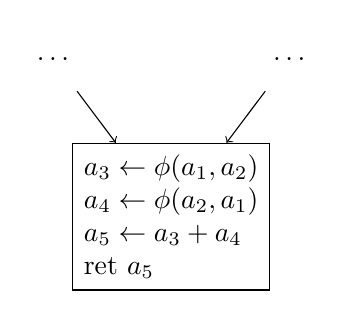
\begin{tikzpicture}
  \node (b1) at (-1.5, 0) [minimum height=0.8cm] {$\dots$};
  \node (b2) at (1.5, 0) [minimum height=0.8cm] {$\dots$};
  \node (end) at (0, -2) [draw, align=left, inner sep=4pt] {$a_3 \leftarrow \phi(a_1, a_2)$ \\ $a_4 \leftarrow \phi(a_2, a_1)$ \\ $a_5 \leftarrow a_3 + a_4$ \\ ret $a_5$};

  \draw[->] (b1) -- (end);
  \draw[->] (b2) -- (end);
  \end{tikzpicture}
\end{minipage}
\hfill
\begin{minipage}{0.48\textwidth}
  \centering
  \caption{Same basic block after \gls{ra} with three physical registers.}
  \label{fig:par2}
  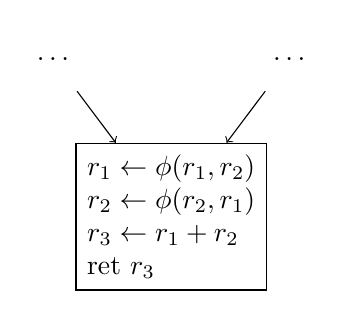
\begin{tikzpicture}
  \node (b1) at (-1.5, 0) [minimum height=0.8cm] {$\dots$};
  \node (b2) at (1.5, 0) [minimum height=0.8cm] {$\dots$};
  \node (end) at (0, -2) [draw, align=left, inner sep=4pt] {$r_1 \leftarrow \phi(r_1, r_2)$ \\ $r_2 \leftarrow \phi(r_2, r_1)$ \\ $r_3 \leftarrow r_1 + r_2$ \\ ret $r_3$};

  \draw[->] (b1) -- (end);
  \draw[->] (b2) -- (end);
  \end{tikzpicture}
\end{minipage}
\end{figure}

\section{\glsentrylong{ra}}
\label{sec:ra}

\gls{ra} assigns a potentially unbounded number of virtual registers to a limited number of physical registers. A well-known approach reduces this problem to graph coloring of the interference graph~\cite{HGG:2006:RA-SSA}. Before talking about this approach, let us introduce some definitions.

\begin{definition}[Liveness]\label{def:liveness}
  Given a \gls{cfg}, a variable $u$ is live at instruction $i$, if $u$ is already defined, and its value may be used by a future instruction.
\end{definition}

\begin{definition}[Interference]
  Given a \gls{cfg}, two variables $u$ and $v$ interfere, iff there exists at least one instruction where they are both live.
\end{definition}

\begin{definition}[Interference Graph]\label{def:ig}
  Given a \gls{cfg}, its interference graph is $G = (V, E)$ where
  \begin{itemize}
  \item $V$ is the set of variables used by the instructions of the \gls{cfg}
  \item $E$ is the set of edges such that $\{ u, v \} \in E$, iff variables $u$ and $v$ interfere.
  \end{itemize}
\end{definition}

By looking at \Cref{def:liveness}, we see that if two variables interfere, they cannot be assigned to the same register. This is because, if they were, one of the two values would be lost.
Now take an interference graph, as defined in \Cref{def:ig}, such that there is an edge between two variables, say $u$ and $v$. Since $u$ and $v$ interfere, they must be assigned different registers.
It is now immediate to see that the problem of \gls{ra} consists in finding a coloring of the interference graph. In this instance of the problem, the nodes are the variables, while the colors are the physical registers.
Take the program shown in \Cref{fig:ig1}, we derive the following interferences:
\begin{itemize}
  \item At line 3, both \texttt a and \texttt b are live, since they are used later at line 4;
  \item At line 4, both \texttt c and \texttt b are live, since they are used later at line 5;
  \item At line 4, both \texttt c and \texttt a are live, since they will be used later, respectively at lines 5 and 6;
  \item Finally, at line 5, both \texttt d and \texttt a are live, since they will be used later at line 6;
\end{itemize}

We use these interferences to build the interference graph in \Cref{fig:ig2}, and we present a valid three-coloring for that graph in \Cref{fig:ig3}. After finding the coloring we translate each variable into its assigned register in \Cref{fig:ig4}.

\begin{figure}[ht]
\centering
\begin{minipage}{0.48\textwidth}
\lstset{style=C}
\begin{lstlisting}[caption={C program returning $2a + 3b$.}, label={fig:ig1}]
int foo() {
    int a = get_a();
    int b = get_b();
    int c = a + b;
    int d = c + b;
    int e = a + d;
    return e;
}
\end{lstlisting}
\end{minipage}
\hfill
\begin{minipage}{0.48\textwidth}
  \centering
  \caption{Interference graph of program shown in \Cref{fig:ig1}.}
  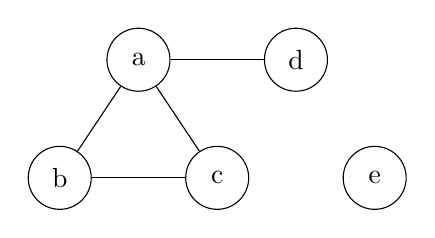
\begin{tikzpicture}[scale=1, every node/.style={circle, draw, minimum size=8mm}]
    \node (a) at (1,1.5)  {a};
    \node (b) at (0,0)      {b};
    \node (c) at (2,0)     {c};
    \node (d) at (3,1.5)    {d};
    \node (e) at (4,0)       {e};

    \draw (a) -- (b);
    \draw (b) -- (c);
    \draw (a) -- (c);
    \draw (d) -- (a);
  \end{tikzpicture}
  \label{fig:ig2}
\end{minipage}
\end{figure}

\begin{figure}[ht]
\centering
\begin{minipage}{0.48\textwidth}
  \centering
  \caption{Three-coloring of the interference graph shown in \Cref{fig:ig2}.}
  \begin{tikzpicture}[scale=1, every node/.style={circle, draw, minimum size=8mm}]
    \node[fill=\cbnodeA!60]  (a) at (1,1.5)  {a};
    \node[fill=\cbnodeB!60]   (b) at (0,0)    {b};
    \node[fill=\cbnodeC!60]  (c) at (2,0)    {c};
    \node[fill=\cbnodeB!60]   (d) at (3,1.5)  {d};
    \node[fill=\cbnodeA!60]  (e) at (4,0)    {e};

    \draw (a) -- (b);
    \draw (b) -- (c);
    \draw (a) -- (c);
    \draw (d) -- (a);
  \end{tikzpicture}
  \label{fig:ig3}
\end{minipage}
\hfill
\begin{minipage}{0.48\textwidth}
\lstset{style=C}
\begin{lstlisting}[caption={{Program shown in \Cref{fig:ig1} after \gls{ra}.}}, label={fig:ig4}, escapeinside={(*}{*)}]
int foo() {
    int (*\textcolor{\cbnodeA}{a}*) = get_a();
    int (*\textcolor{\cbnodeB}{b}*) = get_b();
    int (*\textcolor{\cbnodeC}{c}*) = (*\textcolor{\cbnodeA}{a}*) + (*\textcolor{\cbnodeB}{b}*);
    int (*\textcolor{\cbnodeB}{d}*) = (*\textcolor{\cbnodeC}{c}*) + (*\textcolor{\cbnodeB}{b}*);
    int (*\textcolor{\cbnodeA}{e}*) = (*\textcolor{\cbnodeA}{a}*) + (*\textcolor{\cbnodeB}{d}*);
    return (*\textcolor{\cbnodeA}{e}*);
}
\end{lstlisting}
\end{minipage}
\end{figure}

\subsection{\glsentrylong{ra} in SSA Form}
\label{subsec:ssara}

Before talking about \gls{ra} in SSA form we need to define some properties of nodes and graphs.

\begin{definition}[Clique]\label{def:clique}
  Given a graph $G = (V, E)$, and $C \subseteq V$, we say that $C$ is a clique of $G$, iff for every $u, v \in C$, where $u \neq v$, there exists an edge $\{ u, v \} \in E$.
\end{definition}

\begin{definition}[Simplicial Node]\label{def:simplicial}
  Given a graph $G = (V, E)$, a node $u \in V$ is simplicial in $G$, iff the neighborhood of $u$ is a clique of $G$.
\end{definition}

\begin{definition}[\gls{peo}]\label{def:peo}
  Given a graph $G = (V, E)$, a \gls{peo} is permutation of the nodes, $u_1, u_2, \dots, u_n$, such that $u_1$ is simplicial in $G$, $u_2$ is simplicial in $G - u_1$, \dots, and $u_n$ is simplicial in $(\{ u_n \}, \emptyset)$.
\end{definition}

\begin{definition}[Chordal Graph]\label{def:chordal1}
  A graph for which there exists a \gls{peo}.
\end{definition}

The reason why chordal graphs are particularly appealing are the two following theorems:

\begin{theorem}[Coloring of Chordal Graphs]
  The problem of graph coloring for chordal graphs can be solved optimally and in polynomial time~\cite{golumbic2004algorithmic}.
\end{theorem}

\begin{theorem}[Chordality of \gls{ssa} Programs]
  The interference graph of a program in \gls{ssa} form is chordal~\cite{HGG:2006:RA-SSA}.
\end{theorem}

From these, follows that, while \gls{ra} is NP-complete for arbitrary representations, this problem becomes solvable optimally and in polynomial time for programs in \gls{ssa} form.

% TODO: more buildup
Here we introduce some other definitions that we will use later, during the description of the algorithm.

\begin{definition}[Chromatic Number]\label{def:chromatic}
  Given a graph $G = (V, E)$, its chromatic number $\omega(G)$ is the minimum number of colors that can be assigned to the nodes of $G$ such that no two adjacent nodes have the same color.
\end{definition}

\begin{theorem}[Chromatic Number of Chordal Graphs]\label{thm:chordal-chromatic}
  Given a chordal graph $G$, its chromatic number is equal to the size of the largest clique in $G$~\cite{golumbic2004algorithmic}.
\end{theorem}